\documentclass[10pt,a4paper]{article}
\usepackage[T1]{fontenc}\usepackage{lmodern}
\usepackage[margin=22mm,headheight=14pt]{geometry}
\usepackage{amsmath,amssymb,bm,booktabs,tabularx,array,graphicx,float,fancyhdr,microtype,xcolor}
\usepackage[colorlinks=true,linkcolor=blue!45!black,urlcolor=blue!45!black,citecolor=blue!45!black]{hyperref}
\setlength{\parindent}{0pt}\setlength{\parskip}{5pt}\renewcommand{\arraystretch}{1.15}
\pagestyle{fancy}\fancyhf{}\fancyhead[L]{\small QFT Project B | Final report}\fancyhead[R]{\small Group B}\fancyfoot[C]{\thepage}
\newcommand{\dd}{\mathrm{d}}
\begin{document}\hypersetup{pageanchor=false}
\begin{titlepage}\centering\vspace*{3mm}

\includegraphics[width=36mm]{assets/bits_logo.png}\par\vspace{13mm}
{\Large\bfseries BITS PILANI K.K. BIRLA GOA CAMPUS\par}\vspace{3mm}
{\large\bfseries Department of Physics\par}\vspace{18mm}
{\LARGE\bfseries What Quantum Trace Can\\[2mm] a Heavy Particle Leave?\par}\vspace{6mm}
{\large Curvature--Spectator Entanglement\\and the Cosmological Collider\par}\vspace{10mm}
{\large\bfseries Final Research Report\par}\vspace{17mm}
{\Large\bfseries Group-B\par}\vspace{5mm}
\begin{tabular}{ll}Priyansh Rawat & 2023B5A70968G\\Mayank Sinha & 2023B5A70942G\\Samarth Bhatnagar & 2023B5A70853G\end{tabular}
\vfill{\large Under Professor: Rudranil Basu\par}\vspace{7mm}{29 October 2026\par}
\end{titlepage}\setcounter{page}{1}\hypersetup{pageanchor=true}
\section{Abstract and physical question}
We calculate light--spectator Gaussian entanglement and a leading cubic spectator bispectrum in a specified two-field de Sitter model. The aim is to determine whether greater Gaussian entropy implies a stronger or more recoverable heavy-field signal. Independent oscillator, mode-evolution, canonical-commutator and in-in-integral tests establish the implementation. A mass/mixing scan compares entropy at common times. A converged squeezed bispectrum at $M=2$, $g=0.1$ exhibits a logarithmic clock. Mock fits test frequency recovery; physical fits show why background and window variation must supplement a narrow numerical profile. Finally, varying the cubic coupling changes the signal while leaving the quadratic entropy fixed. The result demonstrates that Gaussian entropy alone cannot determine the leading three-point amplitude.
\subsection{Model and conventions}
We set $\hbar=c=1$ and use $a=-1/(H\eta)$, $\eta<0$, $x=-k\eta=k/(aH)$, $M=m/H$ and $g=\rho/H$. Numerically $H=1$. The action is
\begin{align}S_2=\int\dd\eta\,\dd^3x\bigg\{&\frac{a^2}{2}[q'^2-(\nabla q)^2+\sigma'^2-(\nabla\sigma)^2]\\&-\frac{a^4m^2}{2}\sigma^2+a^3\rho q'\sigma\bigg\}.\end{align}
We use $q(\bm{x})=\int\dd^3k\,q_{\bm{k}}e^{i\bm{k}\cdot\bm{x}}/(2\pi)^3$ and define $P_q$ and $B_q$ after removing the momentum-conserving $(2\pi)^3\delta^3$ factors. The dimension-one field $q=C\zeta$ has an unspecified conversion $C$ to curvature; we keep this normalisation explicit. The single-clock curvature reference follows from the dilation response $-(3+k\partial_k)P_\zeta$, with $P_\zeta\propto k^{n_s-4}$:
\begin{equation}\lim_{k_L/k_S\to0}\frac{B_\zeta}{P_\zeta(k_L)P_\zeta(k_S)}=1-n_s=0.035\quad(n_s=0.965).\end{equation}
This specified tilted reference is distinct from the exact de Sitter spectator calculation. It is not inserted into the computed spectator bispectrum.

\newpage
\section{Gaussian benchmark and canonical dynamics}
The two-oscillator ground state with $K=\left(\begin{smallmatrix}1&0.3\\0.3&2\end{smallmatrix}\right)$ has $X=K^{-1/2}/2$ and $P=K^{1/2}/2$. The reduced eigenvalue $\nu=\sqrt{X_{11}P_{11}}$ gives
\begin{equation}s(\nu)=(\nu+\tfrac12)\ln(\nu+\tfrac12)-(\nu-\tfrac12)\ln(\nu-\tfrac12).\end{equation}
The benchmark is $\nu=0.5028165419863$, $s=0.0193599304236$ nats. Zero coupling gives zero entropy; increasing the coupling to 0.6 gives $s=0.06727111385$. Local canonical rescaling leaves the determinant unchanged to $5.6\times10^{-17}$. Direct Gaussian-kernel purity, $\mathrm{Tr}\rho_1^2=1/(2\nu)$, checks the covariance calculation independently.
Derivative mixing changes the momentum: $\pi_q=a^2q'+a^3\rho\sigma$. The Legendre transform is
\begin{equation}H_k=\frac{(\pi_q-a^3\rho\sigma)^2+\pi_\sigma^2}{2a^2}+\frac{a^2k^2}{2}(q^2+\sigma^2)+\frac{a^4m^2}{2}\sigma^2.\end{equation}
The $\rho^2$ term is essential. Two complex mode columns are evolved using canonical equations and, independently, velocity equations in $N=-\ln x$:
\begin{align}\ddot Q+3\dot Q+x^2Q&=-g(\dot\Sigma+3\Sigma),\\\ddot\Sigma+3\dot\Sigma+(x^2+M^2)\Sigma&=g\dot Q,\\\Pi_q&=(\dot Q+g\Sigma)/x^3,\quad\Pi_\sigma=\dot\Sigma/x^3.\end{align}
Identical finite-time initial data give a maximum scaled column difference of $2.010\times10^{-7}$ at the initial comparison tolerance. The symbolic Legendre-transform identity is exact. Production tests then use tighter tolerances and controlled initial states.
For $V=\operatorname{Re}(\mathcal M\mathcal M^\dagger)$, the full state has symplectic eigenvalues $1/2$, while the light subblock can have $\nu_q>1/2$. Entropies are per real sector; the identical cosine and sine sectors of a nonzero $\pm\bm{k}$ pair contribute twice this entropy.

\newpage
\section{Free modes and the ultraviolet state}
The uncoupled light mode is $Q=(1-ix)e^{ix}/\sqrt2$. The heavy mode is
\begin{equation}\Sigma=\frac{\sqrt\pi}{2}e^{i\pi(\nu/2+1/4)}x^{3/2}H_\nu^{(1)}(x),\qquad\nu=\sqrt{9/4-M^2}.\end{equation}
Complex-order Hankel evaluation and its derivative reproduce both fields with scaled errors below $6\times10^{-10}$ in the free test. The light power approaches $1/2$.
\begin{figure}[H]\centering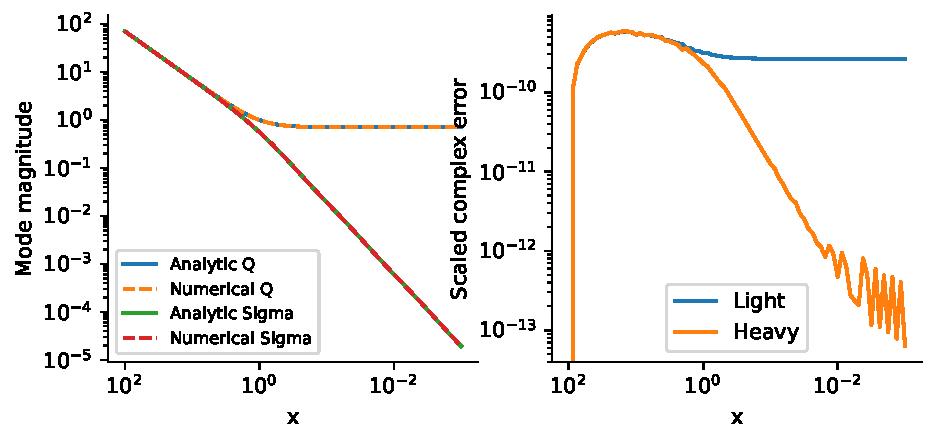
\includegraphics[width=.86\linewidth]{figures/free_modes.pdf}\caption{Free analytic and numerical modes agree in magnitude and complex phase.}\end{figure}A product vacuum imposed at finite $X$ gives visible initial-state contamination in the much smaller bispectrum. We instead construct a positive-frequency ultraviolet state through $Y'=R(x)Y$, $Y=(Q,\Sigma)^T$, with $R=iI+\sum R_n/x^n$. Its Riccati equation follows directly from the coupled field equations. With $J_{12}=1$, $J_{21}=-1$ and $D_{12}=-3g$, $D_{22}=-M^2$,
\begin{equation}R_1=I+gJ/2,\quad 2iR_n=[(n+1)I+gJ]R_{n-1}-\sum_{j=1}^{n-1}R_jR_{n-j}+\delta_{n2}D.\end{equation}
At $X$, choose the position covariance $FF^T=X^2(\operatorname{Im}R)^{-1}/2$ and velocity columns $-XR F$. This imposes canonical initial commutators. Comparing orders 4/6 and $X=100,200,400,800$ verifies the ultraviolet limit. No correction is imposed on the evolved covariance.

\newpage
\section{Gaussian entropy and power}
The benchmark uses sixth-order initial data, $X=400$, relative/absolute tolerances $2.5\times10^{-14}/10^{-17}$ and the local shear $\widetilde\Pi_q=\Pi_q+Q/x$. Extended-precision covariance products reduce late-time cancellation. Samples require commutator residual $<10^{-6}$ and full-state eigenvalue error $<10^{-5}$.
\begin{figure}[H]\centering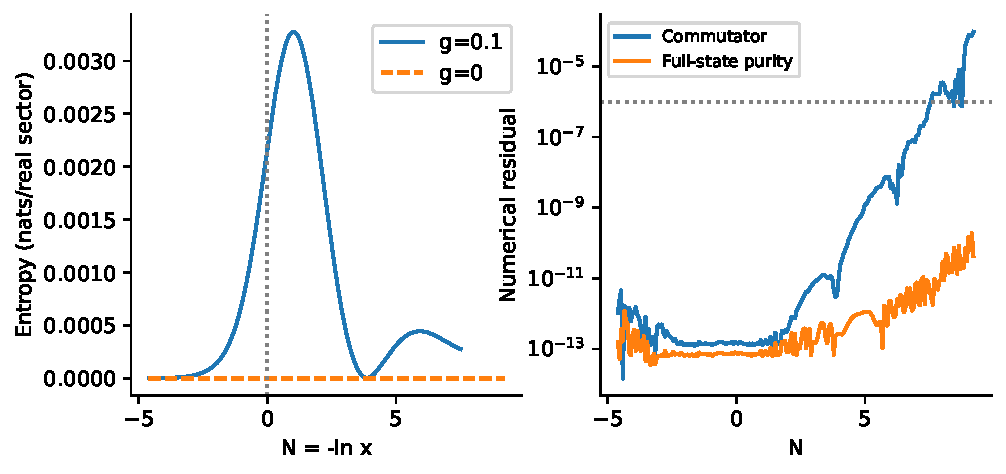
\includegraphics[width=.83\linewidth]{figures/entropy_and_purity.pdf}\caption{Entropy history and purity/commutator diagnostics. The curve stops at the first failure of the numerical criteria.}\end{figure}\begin{figure}[H]\centering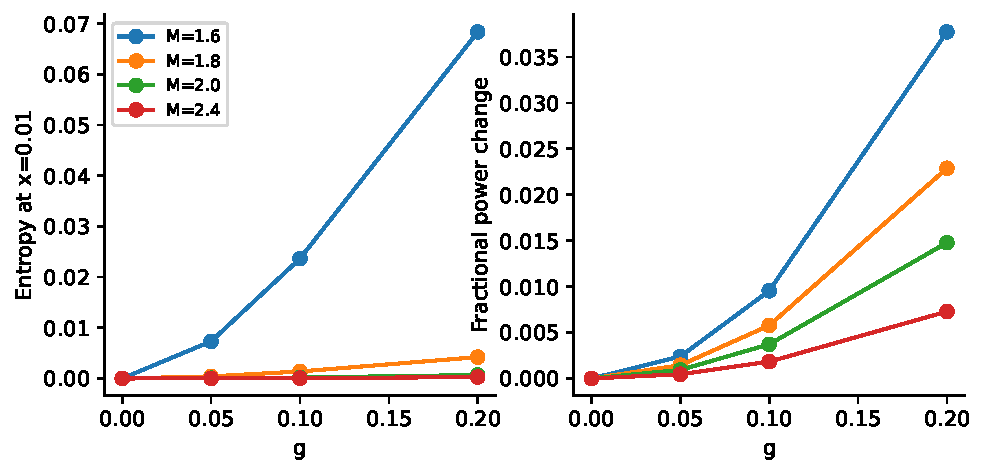
\includegraphics[width=.83\linewidth]{figures/mass_mixing_scan.pdf}\caption{Mass and mixing comparison at $x=0.01$; entropy and power change are separate diagnostics.}\end{figure}All 64 requested mass/mixing/time comparison rows pass. At $M=2$, $g=0.1$, $x=0.01$, $S_q=1.845987\times10^{-4}$ nats and $\Delta P_q/P_{q,0}=0.0037140$. The zero-mixing history has numerical entropy below $2.3\times10^{-9}$; reversing $g$ changes the benchmark entropy by $6.1\times10^{-12}$. Non-monotone entropy evolution is compatible with unitary evolution of the joint pure state. The last reliable contiguous history sample is $x\simeq5.49\times10^{-4}$.

\newpage
\section{In-in test and spectator bispectrum}
At first order in the interaction Hamiltonian,
\begin{equation}\Delta\langle O\rangle=-i\int\dd\eta\,\langle[O,H_I]\rangle_0.\end{equation}
An independent sine quadrature checks the massless test Hamiltonian $H_I=\gamma\int a(q')^3/3!$. Its analytic result is
\begin{equation}B_{\rm test}=-\frac{\gamma H^5}{2k_1k_2k_3(k_1+k_2+k_3)^3}.\end{equation}
The regulated integral is $2/[(\epsilon+i)K]^3$. Equilateral and squeezed tests at $\epsilon=10^{-3}$ agree with the zero-regulator answer to $6.0\times10^{-6}$ relative, meeting the $0.1\%$ requirement.
\begin{figure}[H]\centering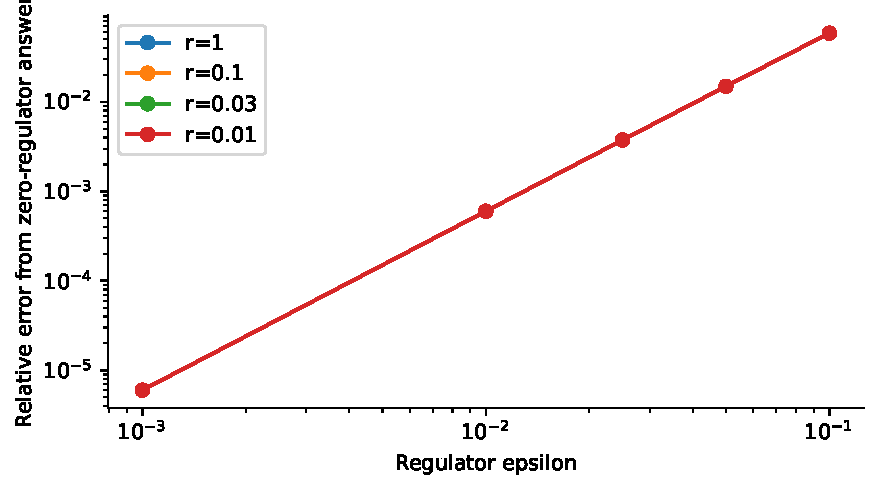
\includegraphics[width=.80\linewidth]{figures/in_in_benchmark.pdf}\caption{Independent oscillatory quadrature reproduces the analytic test and its regulator dependence.}\end{figure}For $H_I=\lambda_3\int a^4\sigma^3/3!$, define $K_k=\sum_a q_k^a(\eta_f)\sigma_k^{a*}(\eta)$. The six contractions cancel $3!$ and the commutator gives
\begin{equation}B_q=2\lambda_3\int\dd\eta\,a^4\operatorname{Im}(K_1K_2K_3),\quad F(r)=\frac{HB_q(r,1,1)}{P_q(r)P_q(1)}.\end{equation}
At a common physical final time the long leg ends at $rz_f$, not $z_f$. We keep the complex contractions, mode columns and cumulative integrals. The $g=0$ and $\lambda_3=0$ controls vanish exactly; doubling $\lambda_3$ doubles $F$, and weak mixing gives the expected $g^3$ scaling.

\newpage
\section{Convergence of the baseline physical signal}
At $M=2$, $g=0.1$, $\lambda_3/H=0.01$, production integration uses $X=1600$ and sixth-order ultraviolet data. We test regulator/cutoff pairs $(0.1,80),(0.05,160),(0.025,320)$ at doubled cutoffs, add $\epsilon=0.0125$, and extrapolate the last three regulators with linear and quadratic models. Early intervals resolve oscillations; late integration uses $\ln z$. Grid refinement and independent adaptive quadrature agree at the $r=0.03$ benchmark to $1.7\times10^{-22}$ in regulated $F$.
Initial $X$, ODE precision, quadrature, regulator, early tail and final time are varied separately. The sum of their changes is a conservative numerical budget, not a statistical error bar.
\begin{center}\small\begin{tabular}{lll}\toprule $r$ & $F$ extrapolated & Numerical budget\\\midrule
$0.2$ & $1.812\times10^{-8}$ & $1.059\times10^{-10}$\\
$0.1$ & $1.585\times10^{-9}$ & $2.857\times10^{-11}$\\
$0.03$ & $-3.986\times10^{-10}$ & $1.104\times10^{-12}$\\
$0.01$ & $6.258\times10^{-11}$ & $2.940\times10^{-13}$\\
$0.003$ & $2.482\times10^{-11}$ & $4.818\times10^{-14}$\\
$0.001$ & $-2.966\times10^{-13}$ & $1.414\times10^{-14}$\\\bottomrule\end{tabular}\end{center}\begin{figure}[H]\centering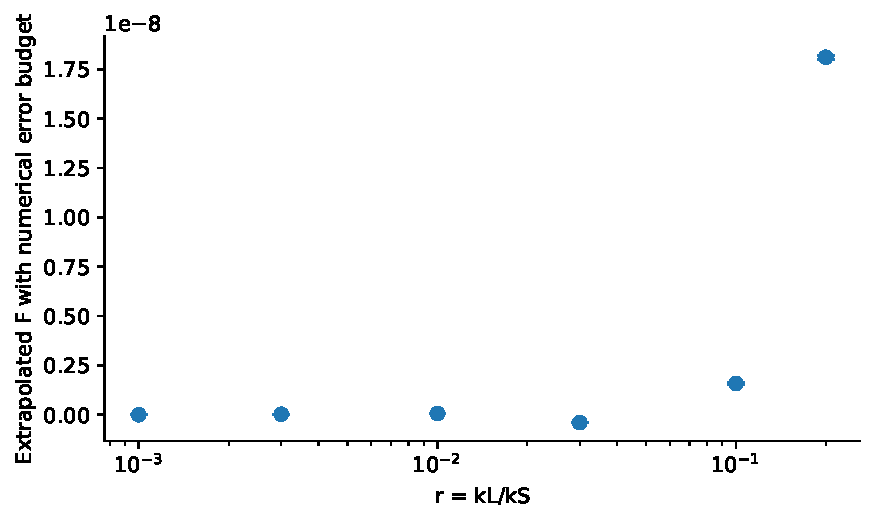
\includegraphics[width=.82\linewidth]{figures/bispectrum_convergence.pdf}\caption{Physical pilot values and the tested numerical budget. Near a clock zero, relative error in the total value can be large while envelope precision remains useful.}\end{figure}The largest pilot error normalised to a clock-envelope scale is $0.00585$. In the 50-point shape scan the largest numerical error is less than 0.009 of the fitted oscillatory envelope. This supports studying the resolved shape while still requiring the fit-window checks below.

\newpage
\section{Mock recovery and no-clock controls}
Outside the horizon the heavy branch behaves as $x^{3/2\pm i\mu}$ with $\mu=\sqrt{M^2+g^2-9/4}$. We profile frequency using
\begin{equation}F=b_0+b_2r^2+r^{3/2}[A\cos(\mu\ln r)+B\sin(\mu\ln r)],\end{equation}
solving linearly for nuisance coefficients at each frequency. The scan covers $0.1\le\mu\le4$ in steps $0.01$, refining every candidate minimum.
The mocks use $M=2$, $g=0.1$, $\mu=1.326649916$, $A=0.1$, $B=0.05$, $b_0=0$, $b_2=0.2$, 50 logarithmic momenta and known independent noise. There are 100 trials at each of 1\% and 5\% oscillatory-RMS noise; the seed is 20261029.
\begin{center}\small\begin{tabular}{llll}\toprule Noise & Frequency RMSE & 95\% coverage & Held-out null false alarm\\\midrule
1\% & $0.04687$ & 93\% & 2\%\\
5\% & $0.205$ & 94\% & 4\%\\\bottomrule\end{tabular}\end{center}\begin{figure}[H]\centering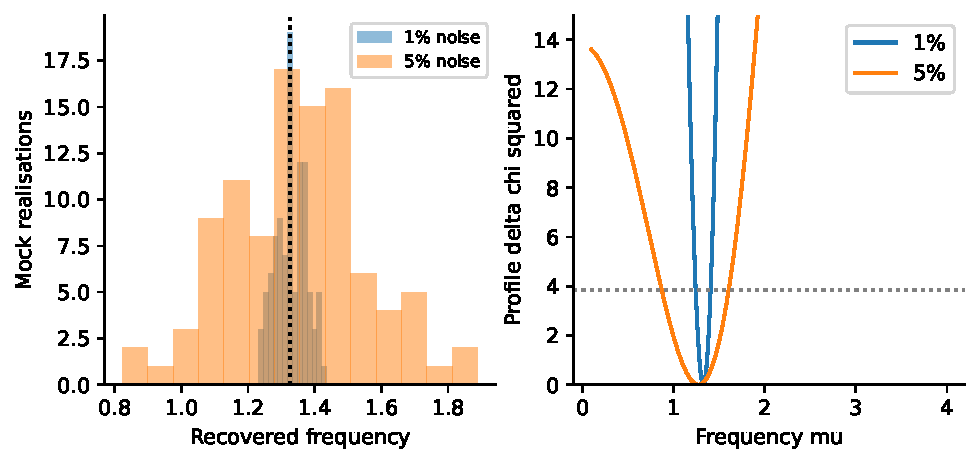
\includegraphics[width=.86\linewidth]{figures/mock_mass_recovery.pdf}\caption{Mock recovered frequencies and profile curves. The likelihood intervals apply to these known Gaussian-noise experiments.}\end{figure}The no-clock thresholds are calibrated on separate null samples and tested on 100 independent null realisations per noise level. These rates have sampling uncertainty of a few percentage points. They explicitly include the search over frequency, which is not identifiable under the no-clock hypothesis.

\newpage
\section{Physical mass assessment}
The converged physical scan uses $10^{-3}\le r\le0.2$. Its numerical errors are used as fit weights, with background and endpoint variations assessed separately. The fitted full-range coefficient amplitude is approximately $1.389\times10^{-7}$, with only 1.11 visible cycles. We convert frequency with
\begin{equation}m/H=\sqrt{\mu^2+9/4-g^2}.\end{equation}
\begin{figure}[H]\centering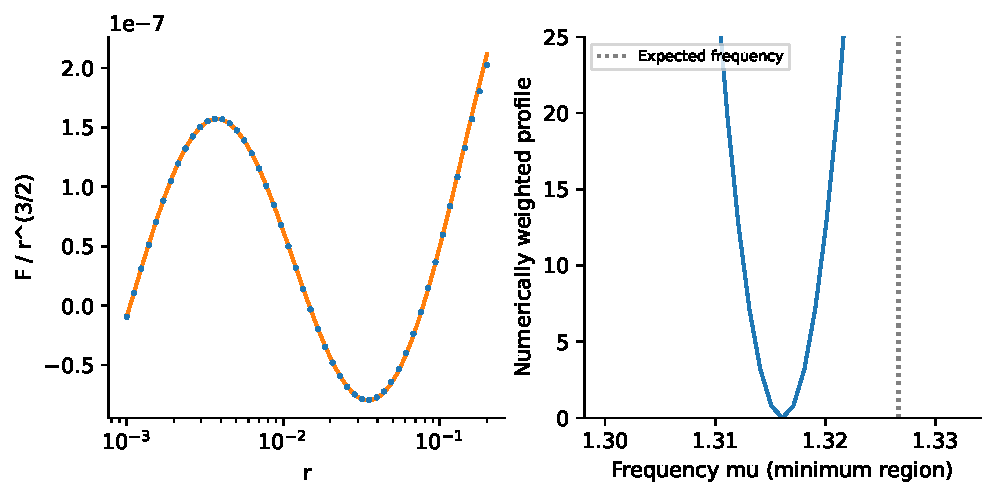
\includegraphics[width=.84\linewidth]{figures/physical_clock_fit.pdf}\caption{Physical squeezed shape and its numerical frequency profile. The narrow profile under one model excludes neither background nor endpoint sensitivity.}\end{figure}\begin{center}\small\begin{tabular}{llll}\toprule $r_{\max}$ & Extra $r^4$ & $\mu$ & $m/H$\\\midrule
$0.05$ & no & $1.32317$ & $1.99769$\\
$0.05$ & yes & $1.32544$ & $1.9992$\\
$0.1$ & no & $1.32041$ & $1.99587$\\
$0.1$ & yes & $1.32445$ & $1.99854$\\
$0.2$ & no & $1.3161$ & $1.99302$\\
$0.2$ & yes & $1.32196$ & $1.99689$\\\bottomrule\end{tabular}\end{center}Including both lower endpoints, $r_{\min}=0.001,0.003$, gives the best-fit frequency envelope $1.3161$--$1.3564$ and mass envelope $1.9930$--$2.0198$. This is model/window sensitivity, not a confidence interval with demonstrated coverage. It contains the input mass $M=2$, but does not justify reporting a highly precise mass from a single narrow profile. If mixing is unknown, the clock identifies the mass--mixing combination rather than $m$ alone.

\newpage
\section{Entropy, cubic coupling and conclusions}
Changing $\lambda_3$ at fixed $M,g$ leaves the Gaussian entropy unchanged and scales the leading bispectrum. The same quadratic entropy therefore accompanies zero, half-strength and full-strength three-point signals.
\begin{figure}[H]\centering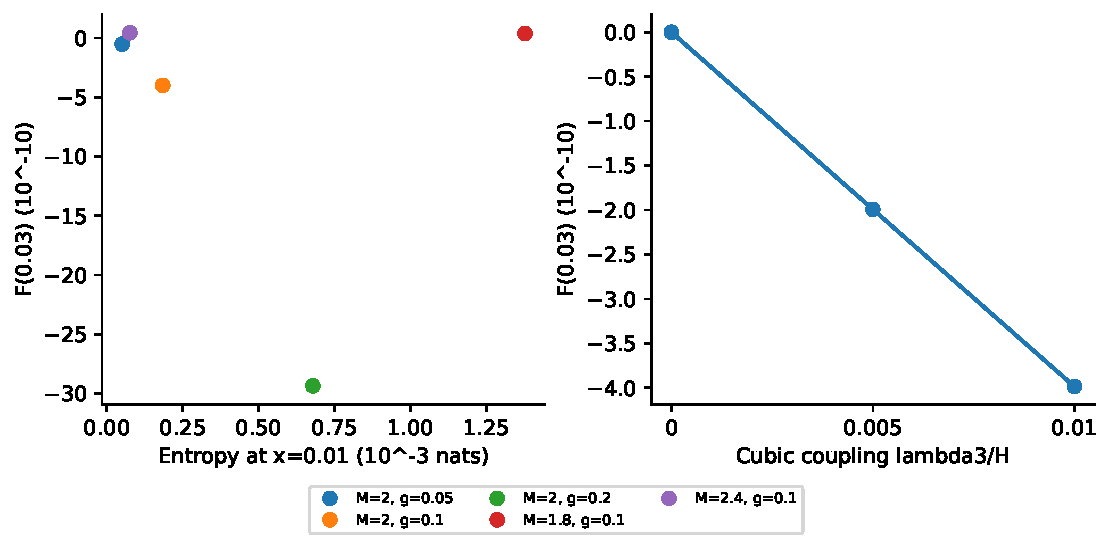
\includegraphics[width=.85\linewidth]{figures/entropy_signal_control.pdf}\caption{Selected entropy--signal points and the independent cubic-coupling control. A single triangle also contains phase information; selected-point bars show regulator variation.}\end{figure}\begin{center}\small\begin{tabular}{lll}\toprule $\lambda_3/H$ & $S_q$ & $F(0.03)$\\\midrule
$0$ & $1.846\times10^{-4}$ & $0$\\
$0.005$ & $1.846\times10^{-4}$ & $-1.993\times10^{-10}$\\
$0.01$ & $1.846\times10^{-4}$ & $-3.986\times10^{-10}$\\\bottomrule\end{tabular}\end{center}This establishes that Gaussian entropy alone cannot determine the spectator three-point amplitude. A fixed-coupling correlation study can still be meaningful, but must hold time, numerical accuracy and measurement covariance fixed. An illustrative fixed covariance $\sigma_F^2I$, $\sigma_F=10^{-10}$, makes known-template signal/noise proportional to the cubic coupling; equal fractional noise would conceal that dependence.
The core calculation has validated entropy, an independent in-in benchmark, a converged baseline bispectrum and an explicit mass-fit stability assessment. Late-time entropy is limited by covariance conditioning; physical mass precision is limited by the available oscillation range and background model. Broader physical amplitude scans are optional extensions. No survey detectability or Bell-test claim follows from these model calculations.
All scripts, inputs, essential tables, complex-mode archives, LaTeX sources and PDF reports are organised by step in the linked repository. Run \texttt{python3 run\_steps.py} after installing the pinned requirements; compile each report from its \texttt{latex/} directory.
\begin{thebibliography}{9}\small
\bibitem{gaussian} C. Weedbrook et al., \emph{Gaussian Quantum Information}, Rev. Mod. Phys. 84, 621 (2012), \href{https://arxiv.org/abs/1110.3234}{arXiv:1110.3234}.
\bibitem{chen} X. Chen and Y. Wang, \emph{Quasi-Single Field Inflation and Non-Gaussianities}, JCAP 04 (2010) 027, \href{https://arxiv.org/abs/0911.3380}{arXiv:0911.3380}.
\bibitem{collider} N. Arkani-Hamed and J. Maldacena, \emph{Cosmological Collider Physics}, \href{https://arxiv.org/abs/1503.08043}{arXiv:1503.08043}.\end{thebibliography}
\textbf{Code and supporting data:} \href{https://github.com/rawatpriyansh17/QFT-PROJECT-GROUP-B/tree/main/final_report}{final\_report on GitHub}.\newpage\section*{Contributions (equal)}\begin{center}\begin{tabularx}{\linewidth}{p{33mm}X}\toprule Member & Contribution\\\midrule Priyansh Rawat & Physical model, canonical derivations and interpretation.\\[3mm]Samarth Bhatnagar & Gaussian validation, convergence controls and mass-fit review.\\[3mm]Mayank Sinha & Numerical implementation, figures and reproducible report assembly.\\\bottomrule\end{tabularx}\end{center}\end{document}